\documentclass[times, utf8, diplomski, numeric, english]{fer}

\usepackage{booktabs}
\usepackage{amsmath}
\usepackage{nccmath}
%\usepackage{hyperref}
\usepackage[section]{placeins}

\usepackage{footnote}
\usepackage{graphicx}

\usepackage{makecell}

\renewcommand\theadalign{cb}
\renewcommand\theadfont{\bfseries}
\renewcommand\theadgape{\Gape[4pt]}
\renewcommand\cellgape{\Gape[4pt]}


\DeclareMathOperator*{\argmin}{\arg\!\min}
\DeclareMathOperator*{\argmax}{\arg\!\max}
\begin{document}


\thesisnumber{1417}
\title{Deep Learning Model for Base Calling of MinION Nanopore Reads}
\author{Marko Ratković}

\maketitle

% Ispis stranice s napomenom o umetanju izvornika rada. Uklonite naredbu \izvornik ako želite izbaciti tu stranicu.
\izvornik

% Dodavanje zahvale ili prazne stranice. Ako ne želite dodati zahvalu, naredbu ostavite radi prazne stranice.
\zahvala{Thanks ...}

\tableofcontents
\listoffigures
\listoftables

%%%%%%%%%%%%%%%%%%%%%%%%%%%%%%%%%%%%%%%%%%%%%%%%%%%%%%%%%%%%%%%%%%%%%%%%%%%%%%%%%%%%%%%
%% CHAPTER
\chapter{Introduction}

In recent years,  deep learning and usage of deep neural networks have significantly improved the state-of-the-art in many application domains such as computer vision, speech recognition, and natural language processing\cite{LeCun:1998:CNI:303568.303704}\cite{NIPS2012_4824}. 
In this thesis, we present application of deep learning in the fields of Biology and Bioinformatics for analysis of DNA sequencing data. 

DNA is a molecule that makes up the genetic material of a cell responsible for carrying the information an organism needs to survive, grow and reproduce. 
It is a long polymer of simple units called nucleotides attached together to form two long strands that spiral to create a structure called a double helix. The order of these bases is what determines DNA's instructions, or genetic code.

DNA sequencing is the process of determining this sequence of nucleotides. Originally sequencing was very expensive process but 
during the last couple of decades, the price of sequencing drastically dropped. A significant breakthrough occurred in May 2015 with the release of MinION sequencer by Oxford Nanopore making DNA sequencing inexpensive and available even for small research teams. 

Base calling is a process assigning sequence of nucleotides (bases) to the raw data generated by the sequencing device or sequencer. Simply put, it is a process of decoding the raw output from the sequencer.


\section{Objectives}
Goal of this thesis is to show that the accuracy of base calling is dependent on the underlying software and can be improved using machine learning methods. Novel approach for base calling of raw data using convolutional neural networks is presented.

\section{Organization}
\indent Chapter 2 gives more detailed explanation of the problem, background on nanopore sequencing and overview of state-of-the-art basecallers.

Chapter 3 describe used deep learning concepts in detail used later on in later chapters.

Chapter 4 goes into implementation details, training of the deep learning model and explains methods used to evaluate obtained results. 

Chapter 5 consists of the results of testing performed on different datasets as well as comparison with state-of-the-art basecallers.

In the end, the Chapter 6 gives a brief conclusion and possible future work and improvements of the developed basecaller.

%%%%%%%%%%%%%%%%%%%%%%%%%%%%%%%%%%%%%%%%%%%%%%%%%%%%%%%%%%%%%%%%%%%%%%%%%%%%%%%%%%%%%%%
%% CHAPTER
\chapter{Background}

\section{Sequencing}

Sequencing the entire genome of an organism is a difficult problem due to limitations of technology.
All sequencing technologies to date have constraints on the length of the strand they can process. 
These lengths are much smaller than the genome for a majority of organisms, therefore, whole genome shotgun sequencing approach is used. 
In this approach, multiple copies of the genome are broken up randomly into numerous small fragments that can be processed by the sequencer. Sequenced fragments are called reads.

Genome assembly is the process of reconstructing the original genome from reads and usually starts with finding overlaps between reads.
The quality of reconstruction heavily depends on the length and accuracy of the reads produced by the sequencer. Short reads make resolving repetitive regions practically impossible.

Figure \ref{fg:sequencing} depicts process of sequencing.

\begin{figure}[!ht]
	\begin{center}
		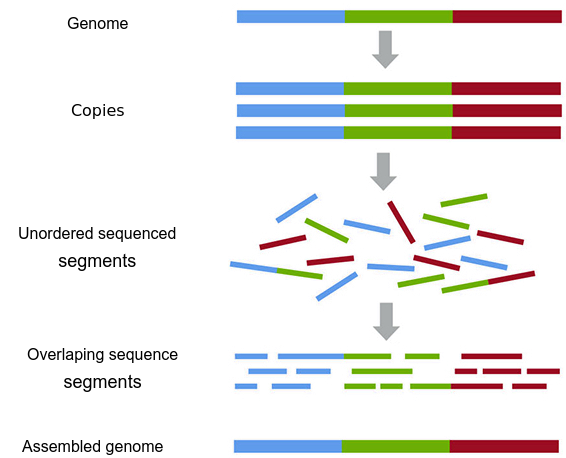
\includegraphics[width=0.6\textwidth]{./imgs/sequencing.png}
		\caption{Depiction of the sequencing process}
		\label{fg:sequencing}
	\end{center}
\end{figure}


Development of sequencing started with work of Frederick Sanger\cite{mile}\cite{Pettersson2009}. In 1977, he developed the first sequencing method which allowed 
read lengths up to 1000 bases with very high accuracy (99.9\%) at a cost of 1\$ per 1000 bases[mile\_skripta].
Second generation sequencing (IAN Torrent and Illumina devices) reduced the price of sequencing while maintaining high accuracy. Mayor disadvantage of these devices is read length of only a few hundred base pairs.
The need for technologies that would produce longer reads led to the development of so-called third generation sequencing technologies.
PacBio developed sequencing method that allowed read lengths up to several thousand bases but at a cost of accuracy. Error Rates of PacBio devices are ~10-15\%. 

Cost makes the main obstacle stopping widespread genome sequencing.
A significant breakthrough occurred in May 2015 with a release of MinION sequencer by Oxford Nanopore making sequencing drastically less expensive and even portable.


\section{Oxford Nanopore MinION}


The MinION device by Oxford Nanopore Technologies (referenca) is the first portable DNA sequencing device.

It’s small weight, low cost, and long read length combined with high-throughput and decent accuracy yield promising results in various applications such as monitoring infectious disease outbreaks [2][3], characterizing structural variants in cancer[4], full human genome assembly [5] what could potentially lead to personalized genomic medicine.



\subsection{Technology}
As its name says, nano-scale pores are used to sequence DNA. An electrical potential is applied over an insulating membrane in which a  pore is inserted. As the DNA passes through the pore, the sensor detects changes in ionic current caused by differences in the shifting nucleotide sequences occupying the pore. Figure \ref{fg:nanopore} shows change of ionic current as DNA strain being pulled through a nanopore.

\begin{figure}[!ht]
	\begin{center}
		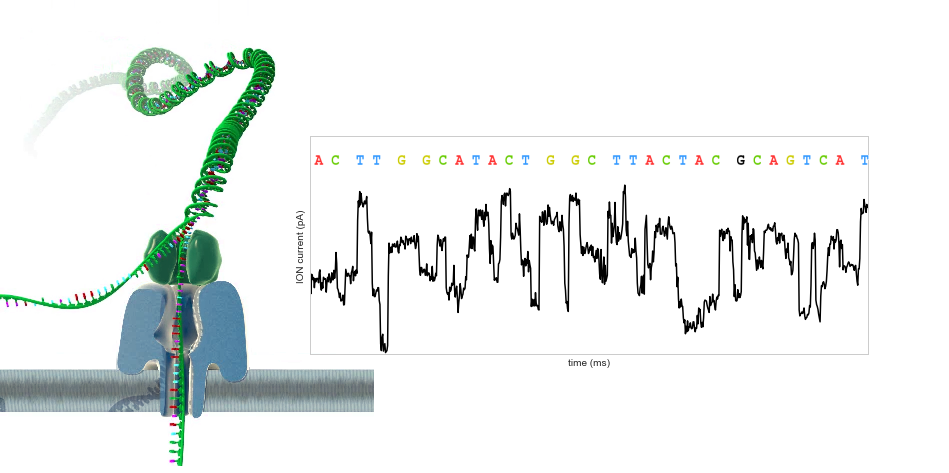
\includegraphics[width=0.8\textwidth]{./imgs/nanopore.png}

		\caption[DNA strain being pulled through a nanopore]{DNA strain being pulled through a nanopore \protect\footnotemark}
		\label{fg:nanopore}
	\end{center}
\end{figure}
\footnotetext{Figure adapted from https://nanoporetech.com/how-it-works}

Minion offers possiblity of sequencing 1D or 2D reads. 
 If information from only one strand is used, the base-calling is termed 1-directional (1D); whereas a 2D base-calling is performed, if information from both strands is incorporated, which results in higher base quality.
 MinION is able to produce long reads, usually tens of thousand
 base pairs (with reported reads above 100 thousand pairs[loman]), they have a high sequencing error
 
Switch from older R7.3 to newer R9 chemistry increases  accuracy of produced data. Accuracy of 1D data increased from 70\% to 85\% while Accuracy of 2D reads from 88\% to 94\%. video. This increase of accuracy makes 1D reads usable to analysis with benefit of faster sample preparation and faster sequencing than 2D reads.


  
\section{Existing basecallers}

Output of the sequencer is fast5 file. Various fields, including signal.
Picture bla shows structure of fast5 file. Analysis fields are added if file is passed to MinKnow for signal segmentation.



\subsection{Official}
Oxford Nanopore  has recently, with R9 version of the platform, introduced a variety of base calling
options. Some of those are production ready and some experimental. Majority of information regarding differences, specifications and similar is only available through community nanoporetech. 
https://community.nanoporetech.com/

Metrichor, a spin-of f of ONT and its main developer of proprietary analysis software, maintains a range of basecallers that haveremained the go-to option for most MinION users. 

Metrichor is an Oxford Nanopore company, offering cloud-based platform EPI2ME for analysis nanopore data. 
Even tho Metrichor is not basecaller but rather the platform, its basecaller is offten called Metrichor for short because to fact that point no local basecallers were available.
Initially, the Metrichor  relied on hidden Markov models (HMM) to find the biological sequence underlying the segmented signal.
Preprocess included segmentation of of the signal into smaller blocks called events defined by my mean value and the variance of the signal in the block, block length and start location of the block in entire signal.

Metrichor than assumed that each event depends on a context of k = 6 consecutive bases and that the context typically shifts by one base in each step. HMM states model context present in the pore and transition correspond to change of bases in the pore. During transition from one state to an other, event is emitted. Basecalling is preformed using Viterbi algorithm which determines most likely sequence of states for the observed sequence of events. Limitatin of this approch is calling homopolymer stretches longer than its k-mer as called bases are determined by difference in two consequitive states.
 
As of early 2016, with release of R9 chemistry, this model was replaced by a more accurate recurrent neural network (RNN)-implementation. Currently Oxford Nanopore offers several RNN-based local basecaller versions under different names; Albacore, Nanonet and the MinKNOW integrated basecaller. Albacore and the MinKNOW version are stable versions intended for regular MinION users.

\textbf{Albacore} is basecaller by Oxford Nanopore Technologies ready for production and activly supported.
The source code of Albacore was not provided and is only available as a binary through the ONT Developer Channel to users who have signed the Developer terms and conditions. 

\textbf{Nanonet}\footnote{\url{https://github.com/nanoporetech/nanonet/}} uses the same neural network that is used in Albacore but it is continually under development. As such, it does not contain production code features such as error handling or logging. It uses CURRENNT library for running neural networks.


\textbf{Scrappie}\footnote{\url{https://github.com/nanoporetech/scrappie}} is an other basecaller by Oxford Nanopore Technologies. Simillar to NanoNet, it is platform for ongoing development. Scrappie was the first basecaller reported to specifically address homopolymer basecalling. It became publicly available just recently in June, 2017.

\subsection{Third-party}



\textbf{Nanocall}\cite{David046086} was the first third-party open source basecaller for nanopore data. It uses HMM approch like the original R7 Metrichor. Metrichor. It uses the segmented signal from minKNOW and assigns k-mers to the events using a hidden Markov model. Nanocall does not support newer chemistries after R7.3.
 

\textbf{DeepNano}\cite{Boza2017}  was the first open-source basecaller based on neural networks that uses bidirectional recurent neural networks. DeepNano was written in Python, using the Theano library. When released, originaly supported R7 chemistry, but support for R9 and R9.4 was added recently.


\begin{figure}[!ht]
	\begin{center}
		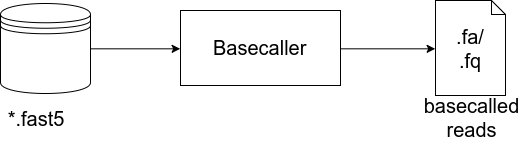
\includegraphics[width=0.5\textwidth]{./imgs/basecalling.png}
		\caption{Basecalling}
		\label{fg:basecalling}
	\end{center}
\end{figure}
%%%%%%%%%%%%%%%%%%%%%%%%%%%%%%%%%%%%%%%%%%%%%%%%%%%%%%%%%%%%%%%%%%%%%%%%%%%%%%%%%%%%%%%
%% CHAPTER
\chapter{Methods}
Process of basecalling can be represented as problem of machine translation where sentence is translated from one language (sequence of events or sequence of current measurements) to an other (sequence of nucleotides). 

This section explaines some key concepts in deep learning needed to understand final model. It gives general idea behind recurrent neural networks and possible problems that serve as motivation for the different approach, usage of convolutional neural networks. 

\section{Arhitecture}

\subsection{RNN}
Recurrent neural networks can be viewed as a simple feed-forward network with the twist that the current output does not only depend on the current input but previous inputs as well. RNNs store that information in their hidden state and that state is updated each step. The figure shows simple RNN and the same RNN unfolded in time.  Unrolling is simple way of showing how network processes each input in the sequence and updates it's hidden state and is shown in figure  \ref{fg:rnn}. 
\begin{figure}[!ht]
	\begin{center}
		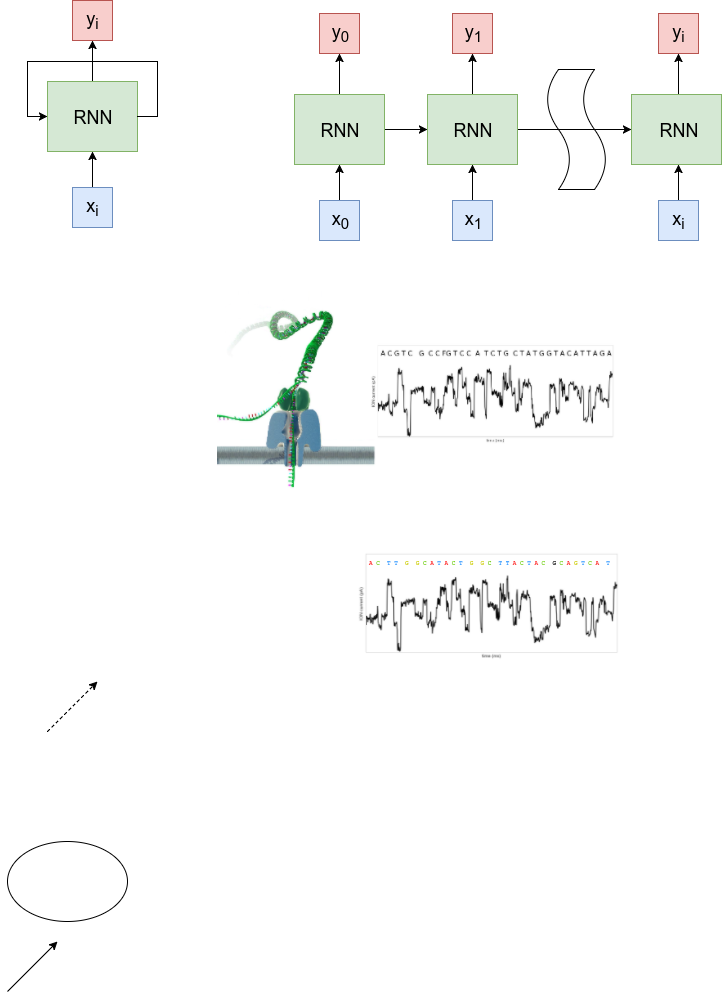
\includegraphics[width=0.8\textwidth]{./imgs/rnn.png}
		\caption{An unrolled recurrent neural network}
		\label{fg:rnn}
	\end{center}
\end{figure}

These networks are trained using a variant of backpropagation called backpropagation through time which is essentially the same as classical backpropagation on an unfolded network. The gradient is propagated through the entire recurrence relation and the gradient is multiplied in each step with the same factor, depending on a scale it can make gradient vanish (drop to 0) or exponentially grow each step and explode. These issues are called the vanishing and exploding gradient\cite{rnn-blog} and are generally resolved by a variant of RNN called \textit{LSTM}\cite{hochreiter1997long}. To take into account dependencies of both previous inputs and next inputs in the sequence bidirectional networks (\textit{BRNN}) are used.  Idea is to combine two RNN (one in the positive direction, one in negative time direction) and have an output of the current state expressed as a function of hidden states of both RNN and current input. This is the approach used in DeepNano\cite{Boza2017}. 


One of the major drawbacks of this kind of networks is computation time. RNN operate sequentially, the output for the second step depends on the first step and so on, which makes parallelization capabilities of RNN quite limited. This especially goes for Bidirectional RNN.

\subsection{CNN}
Convolutional Neural Networks (CNNs) were responsible for major breakthroughs in Image Classification and are the core of most Computer Vision systems today. More recently CNNs are  applied being to problems in Natural Language Processing and have premising results \cite{bytenet}\cite{facebook}.

Easiest way to understand a convolution is by thinking of it as a sliding window function applied to a matrix or in case of signal processing vector. The sliding window is called a kernel or a filter.  Figure \ref{fg:convolution} shows example of convolution with kernel size 3 and how output is calculated as sum of element-wise multiplication of kernel elements and input vector. Stride defines by how much filter is shifted at each step. By how much the window is moved is step of the convolution and it is called stride. Usually to preserve the same dimension, padding is added to the borders. 

\begin{figure}[!ht]
	\begin{center}
		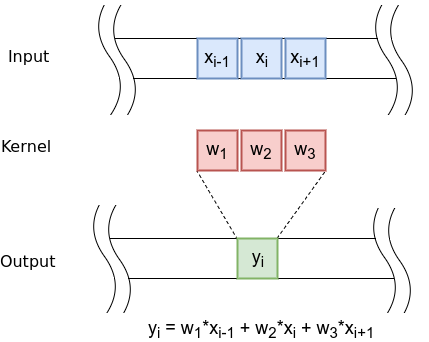
\includegraphics[width=0.5\textwidth]{./imgs/convolution.png}
		\caption{Convolution layer, kernel size 3 with with stride 1.}
		\label{fg:convolution}
	\end{center}
\end{figure}


\subsubsection{Activations}
 After each convolution layer usually nonlinear layer (or activation layer) is applied. The purpose of this layer is to introduce nonlinearity to a system that basically has just been computing linear operations during the conv layers (just element wise multiplications and summations). In classical neural networks, nonlinear functions like tanh and sigmoid were often used, due to undesirable property of saturation(at either tail of 0 or 1 for sigmoid, -1 or 1 for tanh), other activations are used with these networks. 
ReLU. The Rectified Linear Unit has become very popular in the last few years. It computes the function f(x)=max(0,x). In other words, the activation is simply thresholded at zero (see image above on the left).
 It was found to greatly accelerate the convergence of stochastic gradient descent compared to the sigmoid/tanh functions \cite{NIPS2012_4824} and is computationaly efficiant to calculate.

\begin{equation}
ReLU(x) =
	\begin{cases}
		x, & \text{if}\ x>0 \\
		0, & \text{otherwise}
	\end{cases} \\
\end{equation}


Downside of ReLU saturation to the 0 on one side. Once in this state, neuron is unlikely to recover, because the function gradient at 0 is also 0, so gradient descent learning will not alter the weights. This is the problem known as \textit{dying ReLU}.
Different variants of ReLU, PrRelu and ELU are often used to resolve this problem\cite{prelu}\cite{elu}.  

\begin{equation}	
PrELU(x)=
\begin{cases}
x, & \text{if}\ x>0 \\
\alpha x, & \text{otherwise}
\end{cases}\\
\end{equation}
\begin{equation}
ELU(x)=
\begin{cases}
x, & \text{if}\ x>0 \\
\alpha (exp(x) - 1), & \text{otherwise}
\end{cases}	\\
\end{equation}

Figure \ref{fg:activations} show different activation functions.
\begin{figure}[!htb]
	\begin{center}
		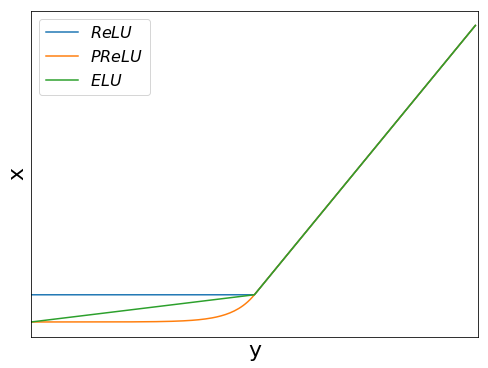
\includegraphics[width=0.5\textwidth]{./imgs/activations.png}
		\caption{Activation functions}
		\label{fg:activations}
	\end{center}
\end{figure}



\subsubsection{Pooling}

The pooling layer is usually placed after the Convolutional layer. Its primary utility lies in reducing the spatial dimensions of the input for the next Convolutional Layer while keeping the most salient information.
Pooling also provides basic invariance to translating (shifting).

 Much like the convolution operation performed above, the pooling layer takes a sliding window or a certain size that is moved in stride across the input transforming the values. Usually transformation is performed by taking the maximum value from the values observable in the window (max pooling).
Figure \ref{fg:pooling} show dimensionality reduction by pooling by factor of 2 using pool of size 2 with stride 2.
\begin{figure}[!htb]
	\begin{center}
		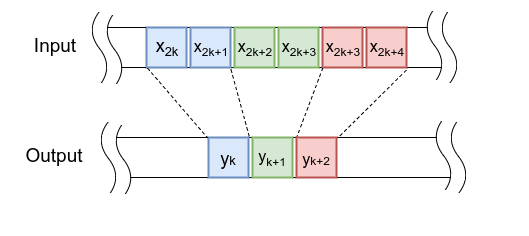
\includegraphics[width=0.5\textwidth]{./imgs/pooling.png}
		\caption{Dimensionality reduction by pooling, kernel size 2, stride 2}
		\label{fg:pooling}
	\end{center}
\end{figure}




  
\subsubsection{Comparision with RNN}

During calculation, each \textit{patch} a convolutional kernel operates on is independent of the other meaning that the entire input layer can be processed concurrently which makes CNNs more efficient than RNNs. 

When compered with RNN, in which output can depend on the entire sequence in convolution layer if depends only on limited spatial information in previous layer defined by kernel size. This is called receptive field of the convolution. 
 Figure \ref{fg:receptive field} shows each new layers depends on larger portion of the input($z_i$ \textit{sees} 5 elements of input). This means that by stacking convolutions sequentialy, later layers can see more of the original input.


\begin{figure}[!ht]
	\begin{center}
		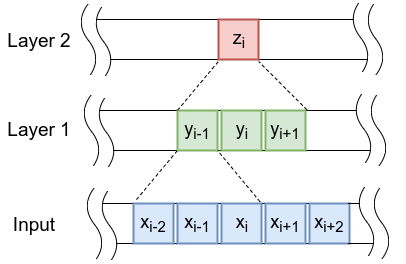
\includegraphics[width=0.5\textwidth]{./imgs/receptive_field.png}
		\caption{Receptive field after 2 layers of convolutions with kernel size 3}
		\label{fg:receptive field}
	\end{center}
\end{figure}

To calculate final output, input signal has to pass throuh entire network but as calculations at each layer happen concurrently and each individual computation is small resulting that in peactice CNNS have a big speed up over RNNS especcialy when dealing with large sequences..

As previously show, stacking layers increases receptive field which makes. In the forward pass input flows and transforms, hopefully becoming a representation that is more amenable to our task. During the back phase we propagate a signal, the gradient, back through the network. Just like in RNNs, that signal gets multiplied and depending on the scales it can vanish. Result of that is no gradient flowing to lower layers and no parameter upgrades. On the one hand, we’d like to be able to take in as much context as possible. On the other hand, if we try to increase our receptive fields by stacking layers we risk vanishing gradients and a failure to learn anything. Resnet arhitecture\cite{resnet} with its residual layes address this issue.



\subsection{Residual Networks}
A Residual Network or ResNet is a neural network architecture which solves the problem of vanishing gradients using simple trick.  
Figure \ref{fg:resnet_block}  shows on the left classical CNN that takes input and transforms it using convolution layers and activation.  This can be representend as function $ H(x) $. 
$ H(x) $ can be written as as sum of some function $F(X)$ and $X$. $  F(X) $ is called the residual.
\begin{figure}[!ht]
	\begin{center}
		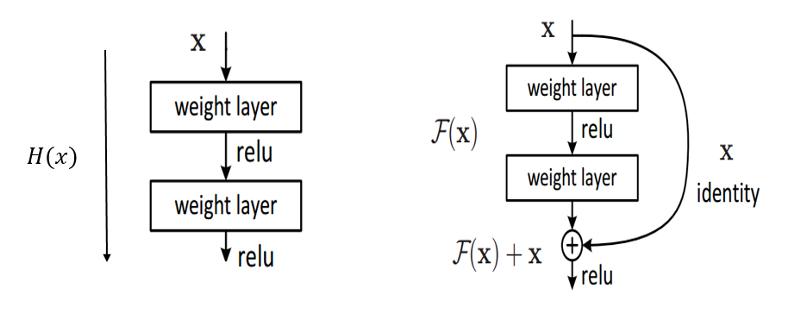
\includegraphics[width=0.7\textwidth]{./imgs/resnet_block.png}
		\caption[Comparison between classical CNN and CNN with residual connection ]{Comparison between classical CNN and CNN with residual connection \protect\footnotemark}
		\label{fg:resnet_block}
	\end{center}
\end{figure}
\footnotetext{Figure adapted from the original paper \cite{resnet}}
Instead of learning $H(X)$, network learns residual and at the output $x$ is simply summed up to the $F(x)$ as shown in the figure. 

By stacking these layers, the gradient could theoretically \textit{skip} over all the intermediate layers and reach the bottom without vanishing.



\section{CTC Loss}

The goal is to design model which can convert from a sequence of events of current measurements into a sequence of base pairs.

Suppose that we have an input sequence $X$ (signal data) and the desired output sequence $Y$ (nucleotides). $X$ and $Y$ will be of different lengths(the length of base pairs is always smaller than the length of the raw signal), which may pose a problem.

Instead of having a variable size of the output from the neural network, we can limit it to length $m$ and from direct output of the network in some way decode our desired output sequence $Y$. $m$ is the maximal allowed length of output sequence $Y$.
Idea is that the network outputs is fixed width and the variable length sequence is derived from them.
The neural network can be considered to be simply a function that takes in some input sequence $X$ (of length $n$) and generate some sequence $O$ (of length $m$). Note that this generated sequence is not same as output sequence $Y$. 

\subsection{Definition}
They key idea behind Connectionist Temporal Classification(CTC)\cite{Graves:2006:CTC:1143844.1143891} is that instead of directly generating output sequence $Y$ as output from the neural network, we  generate a probability distribution at every output length (from $t$=1 to $t$=$m$) that after \textit{decoding} gives maximum likelihood output sequence $Y$. 
Finally, network is trained by creating an objective function that restricts the maximum likelihood decoding for a given sequence $X$ to correspond to our desired target sequence $Y$.


Given an input sequence $X$ of length $n$, the network generates some probabilities over all possible labels (A, C, T, and G) with an extra symbol representing a "blank" at each timestep. 

The output generated by the network is called \textit{path}. Path is defined by the sequence of it's elements $\pi = (\pi_1, \pi_2, ..., \pi_m)$.
The probability of a given path $\pi$, given inputs $X$, can then be written as the product of all its forming elements:

\begin{equation}
\begin{gathered}
P(\pi | X) = \prod_{t=1}^{m} o_t(\pi_t), \\
\text{where $o_t(\pi_t)$ is probability of $\pi_t$ being $t^{th}$ element on path $\pi$}
\end{gathered}
\end{equation}

Real output sequence, for given path, is obtained by traversing the path and removing all blanks and duplicate letters. Let $ decode(\pi) $ be the output sequence corresponding to a path $\pi$. The probability of output sequence $Y$ is then the sum of probabilities of all paths that decode to $Y$:
\begin{equation}
\begin{gathered}
P(Y | X) = \sum_{\pi \in decode^{-1}(Y)}^{} P(\pi | X)
\end{gathered}
\end{equation}
\subsection{Objective}
Given the dataset $D = \{(X, Y)\}$, training objective is the maximization of the likelihood of each training sample which corresponds to the minimization of negative log likelihood:

\begin{equation}
\begin{gathered}
L(D) = - \sum_{(X,Y)\in D}^{} ln P(Y | X)
\end{gathered}
\end{equation}


\subsection{Output decoding}
Given the probability distribution $P(Y | X)$ and given input sequence $X$, most likely $Y^{*}$ can be computed.
\begin{equation}
\begin{gathered}
Y^{*} = \argmax_{Y \in L^m} P(Y|X) = \argmax_{Y \in L^m} \sum_{\pi \in decode^{-1}(Y)}^{} P(\pi | X),\\
\text{~where $L^m$ set of all possible sequences over alphabet $L$ }\\
\text{with length less than or equals to $m$}
\end{gathered}
\end{equation}

The probability of a single output sequence $Y$ is the sum of probabilities of all paths that decode to $Y$ and the most probable sequence is needed to be found.
Calculation of all possible sequences is computationally intractable but exist algorithms that approximate decoding. 

One naive possibility is to take the most probable path and say that output sequence corresponds to that path.
This is not necessarily true: suppose we have one path with probability $0.1$ corresponding with sequence $A$, and ten paths with probabilities  $0.05$ each corresponding to sequence $B$. Clearly, label $B$ is preferable overall, since it has an overall probability of $0.5$; however, this naive best path decoding would select label $A$, which has a higher probability than any single path for label $B$.

Better approximations can be calculated using beam search algorithm proposed in paper\cite{graves_decode}.  
Idea behind this approach is tu 

This serves as a brief overview of the method and explains key concepts why it is used. More detailed explanation can be found in original paper\cite{Graves:2006:CTC:1143844.1143891} or various blog post\cite{ctc-blog}.

\section{Batch normalization}
Batch normalization is method proposed in paper\cite{BNORM} that accelerates learning process. 
During training parameters are updated and distribution of outputs of each layers keep changing. Small change in distribution of outputs in early layers can cause drastic change in later layers and those layers need to adapt to the new scale of their inputs. This change of distribution is called the internal covariate shift and results in slows learning.
Proposed solution for this is to center each output from activations of the mini-batch to zero-mean and unit variance. After that learned scale and offset are applied. This process is called batch normalization. 
After training, mean and variance for each activation is computed on the whole training dataset rather than on mini-batches during training. 
Pros of using batch normalization 
Batch normalization offers several advantages other than reducing internal covariant shift. 
If offers more robust learning process by reducing dependance on scale of the parameters and their initial values. This allows usage of larger learning rates and faster learning all together. It is show in the original paper that batch normalisation also regularizes the model that could potentially improve performance of the model.

%%%%%%%%%%%%%%%%%%%%%%%%%%%%%%%%%%%%%%%%%%%%%%%%%%%%%%%%%%%%%%%%%%%%%%%%%%%%%%%%%%%%%%%
%% CHAPTER
\chapter{Implementation}
\section{Deep Learning model}

Final model is residual neural network consisting of 72 residual blocks depicted in figure \ref{fg:model_block}. This is a variant of arhitecture proposed in paper \cite{identitet} with the difference of ELU being used as activation instead of ReLU as it is reported\cite{resnet-elu} to speeds up learning process and improve accuracy as the depth increase. 



It is difficult to discuss actual performance benefit over simple ReLU without more detailed analysis and comparison for this problem. 

Each residual block contains 2 convolution layers making total number of convolution layers 144. Each convolutional layer in this models uses 64 kernels of 3. Pooling with kernel size 2 is used every 48 layers making output 8 times shorter than signal input. This is used to help training by reducing number of required blank labels in the output and reducing computation effort. 

\begin{figure}[!ht]
	\begin{center}
		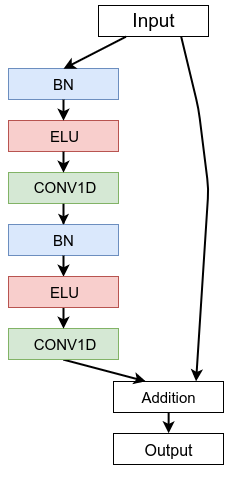
\includegraphics[width=0.2\textwidth]{./imgs/model.png}
		\caption{Used residual block}
		\label{fg:model_block}
	\end{center}
\end{figure}


\section{Training}

To train described model we need to obtain dataset that consist of sample pairs $(X_i, Y_i)$ where $(X_i)$ is input signal and $Y_i$ is output sequence. 
One of the mayor issues is determining correct output for given signal. One option is to use existing basecaller like Metrichor to determine output sequences. 

 

\begin{figure}[!ht]
	\begin{center}
		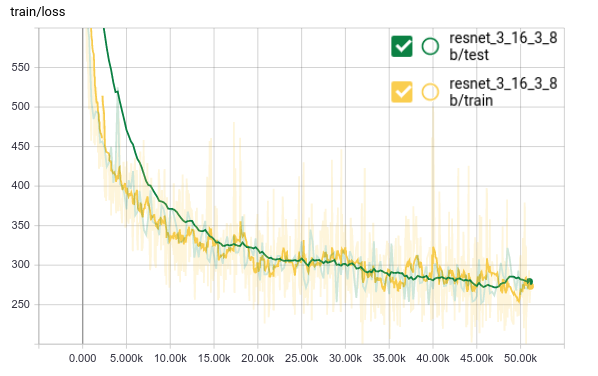
\includegraphics[width=0.6\textwidth]{./imgs/train_tb.png}
		\caption{Learning curve shown in TensorBoard}
		\label{fg:learn}
	\end{center}
\end{figure}


Supervised learning so for need to specify dataset that for each input signal we need specify desired sequence of bases.
{Xi, Yi} where len of X and len of Yi are not specified.

For each input file, ground truth is not specified. If we use output of Metrihor or any other basecaller we limit our model to
obtain accuracy of used basecaller in best case. We limit our train data to only sequencing data of know organisms (organisms with know reference genome) and try to correct data by aligning the read produced by metrichor or any other basecaller to reference genome. Alignment destination is used as target sequencing in training. 
Using Metrichor basecalled data we can determine for each called event values such as start in signal, length of event, k-mer state in the pore and using move field change of k-mer from previous state. 

Used dataset for training consists of raw signal from fast5 files split raw data into blocks of size $l$.
For each block it is easy to determine basecalled events from Metrichor that belong to particular block using start information and from those events basecalled sequence. 


$block\_index =  \frac{event_{start} * sampling\_rate}{block\_size}$

Full basecalled sequence is aligned to the reference genome and alignment was obtained. For each block target sequence is determined from alignment information.

Figure X shows how for given signal block


Figure bla shows augmentation of data.



Gradient descent is one of the most popular algorithms to perform optimization and by far the most common way to optimize neural networks.  Gradient descent is a way to minimize an objective function parameterized by a models parameters  by updating the parameters in the opposite direction of the gradient of the objective function to the parameters.

Adam is a stochastic gradient descent algorithm based on estimation of 1st and 2nd-order moments.
It is often used as it offers fast and stable convergention, even using default arguments proposed by authors.
Learning rate 1e-3 with exponential decay 0.98 every 10000 steps, batch size was set to 8.



To eliminate possibility of overfitting to the know reference, model is trained and tested on reads that align to different regions of reference genome and those regions should not overlap. Also test is conducted on separate set of sequencing data for different organism than the one used for training. 

\begin{figure}[!ht]
	\begin{center}
		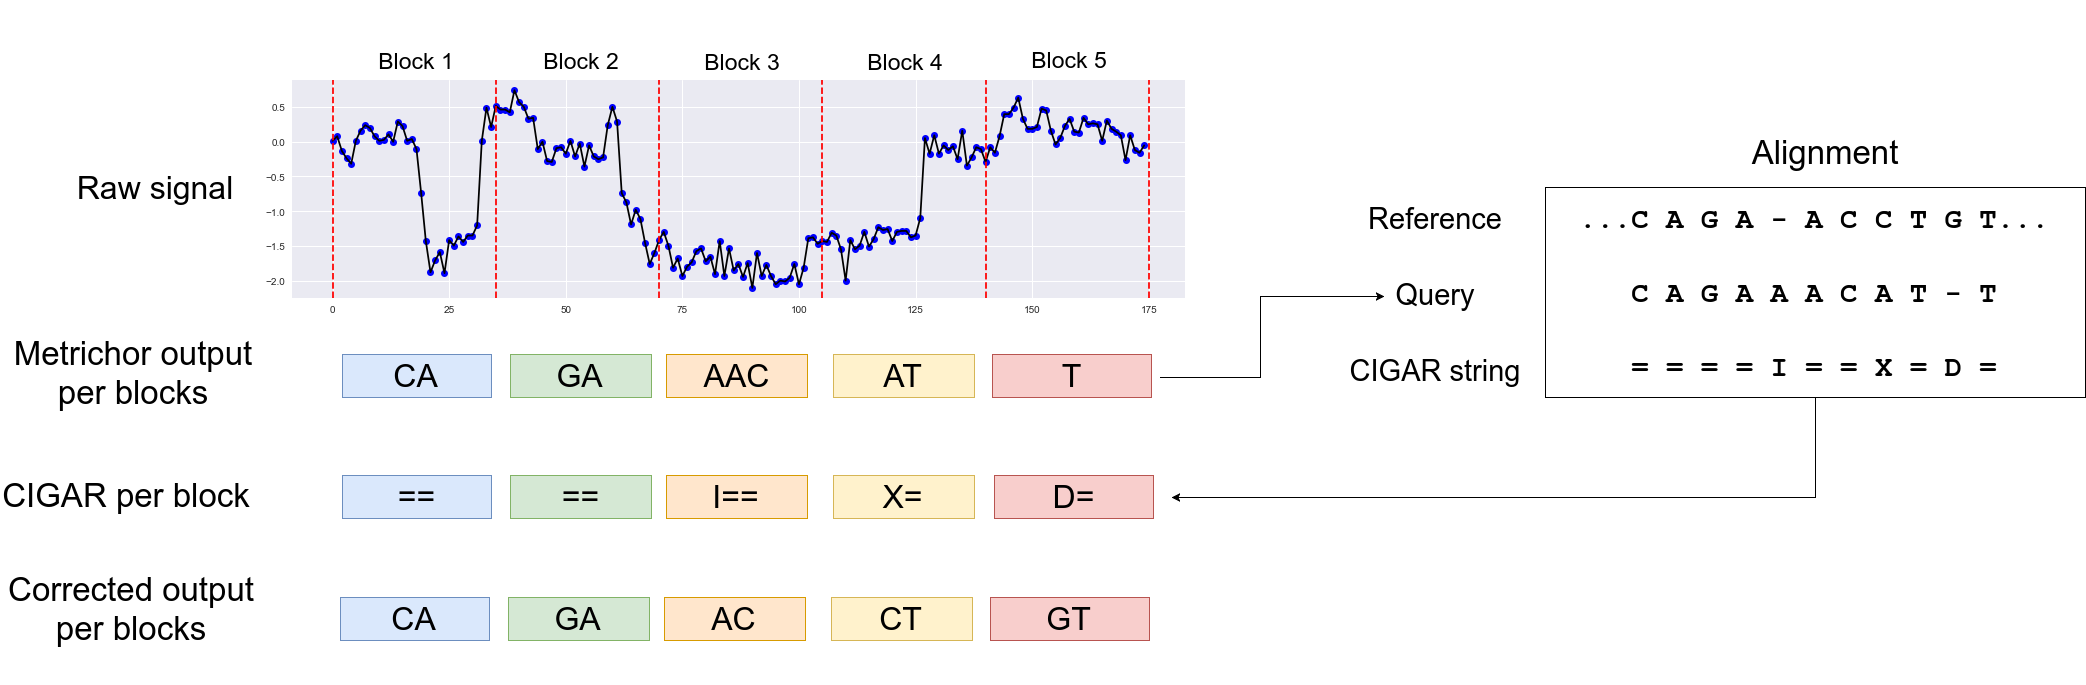
\includegraphics[width=1\textwidth]{./imgs/train_data_correction.png}
		\caption{Dataset preparation}
		\label{fg:data_correction}
	\end{center}
\end{figure}
\begin{figure}[!ht]
	\begin{center}
		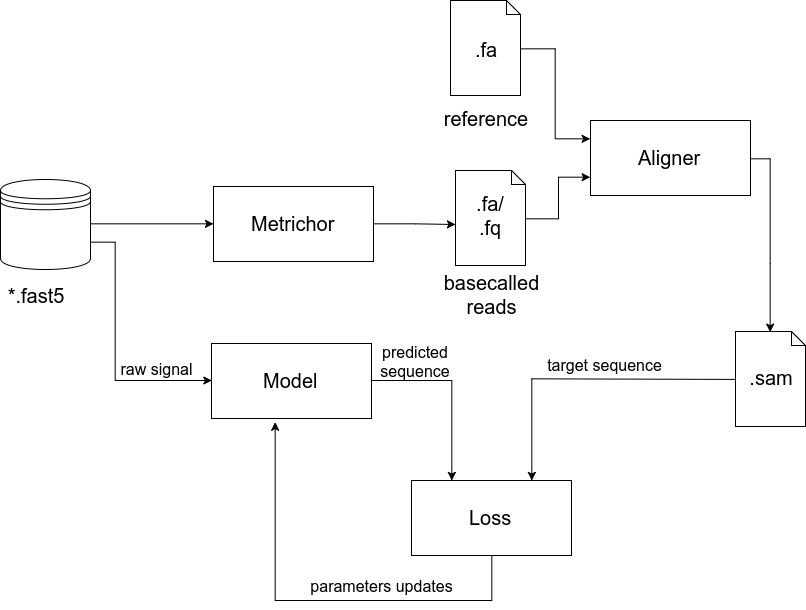
\includegraphics[width=0.7\textwidth]{./imgs/train_pipeline.png}
		\caption{Overview of training pipeline}
		\label{fg:train_pipe}
	\end{center}
\end{figure}
\section{Evaluation methods}
To evaluate trained model we base call test set, align those reads to reference and calculate various statistics on align data.
From cigar string it is easy to calculate following:
the proportion of bases in a sequencing ‘read’ that align to a matching base in a reference sequence

\begin{equation}
\begin{gathered}
read\_len =  n\_matches + n\_missmatches + n\_insertions 
\end{gathered}
\end{equation}
\begin{equation}
\begin{gathered}
match\_rate = \dfrac{n\_matches}{read\_lenght}
\end{gathered}
\end{equation}
\begin{equation}
\begin{gathered}
missmatch\_rate = \dfrac{n\_missmatches}{read\_lenght}
\end{gathered}
\end{equation}
\begin{equation}
\begin{gathered}
insertion\_rate = \dfrac{n\_insertions}{read\_lenght}
\end{gathered}
\end{equation}
\begin{equation}
\begin{gathered}
deletion\_rate = \dfrac{n\_deletion}{read\_lenght}
\end{gathered}
\end{equation}
\begin{equation}
\begin{gathered}
match\_rate = \dfrac{n\_matches}{read\_lenght}
\end{gathered}
\end{equation}

Results are calculated for each read in test dataset and median value, mean and standard deviation is expressed for the whole dataset.

To validate consistency of a basecaller, basecalled data is aligned to the reference genome and consensus sequence is called from all reads covering single position. Consensus sequence is compared with the reference genome and following measures are calculated:
\begin{equation}
\begin{gathered}
identity\_percentage =  100 * \dfrac{n\_correct\_bases}{reference\_lenght}
\end{gathered}
\end{equation}
\begin{equation}
\begin{gathered}
match\_rate = \dfrac{n\_correct\_bases}{consensus\_lenght}
\end{gathered}
\end{equation}
\begin{equation}
\begin{gathered}
snp\_rate = \dfrac{n\_snp}{consensus\_lenght}
\end{gathered}
\end{equation}
\begin{equation}
\begin{gathered}
insertion\_rate = \dfrac{n\_insertions}{consensus\_lenght}
\end{gathered}
\end{equation}
\begin{equation}
\begin{gathered}
deletion\_rate = \dfrac{n\_deletion}{consensus\_lenght}
\end{gathered}
\end{equation}



\begin{figure}[!ht]
	\begin{center}
		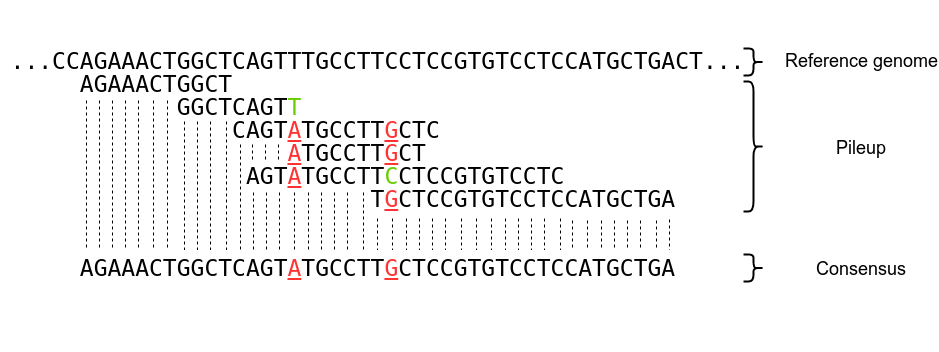
\includegraphics[width=0.8\textwidth]{./imgs/consnesus.png}
		\caption{Consensus from pileup}
		\label{fg:consensus}
	\end{center}
\end{figure}


\begin{figure}[!ht]
	\begin{center}
		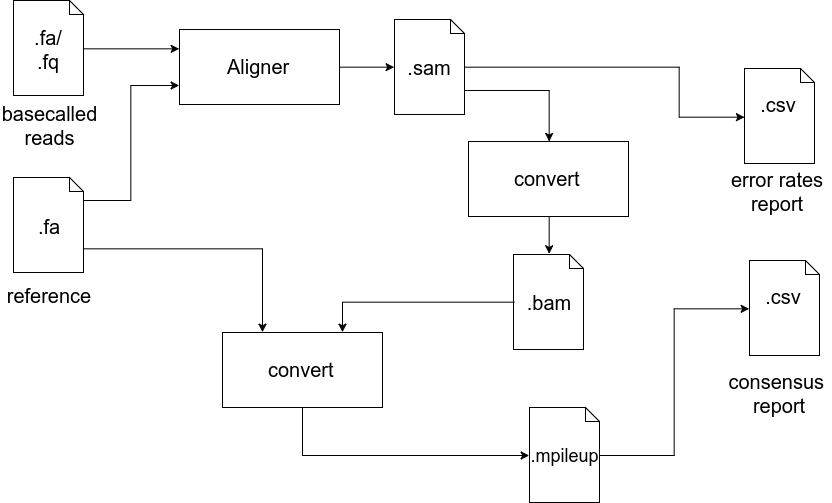
\includegraphics[width=0.7\textwidth]{./imgs/evaluation_pipeline.png}
		\caption{Overview of evaluation pipeline}
		\label{fg:eval_pipe}
	\end{center}
\end{figure}

\section{Technologies}

Overall solution was implemented in Python programing language. Described model is implemented using TensorFlow. It is an open source software library for numerical computation using data flow graphs developed by Google. TensorFlow, even tho is considered low-level framework offers implementations of higher level concepts (layers, losses, and optimizers) which makes it great for prototyping while keeping it modular and extensible for highly specific tasks as well.

TensorFlow offers efficient GPU implementations of various layers and losses but as of version 1.2 lacks GPU implementation of used CTC loss, so WARP-CTC\footnote{\url{https://github.com/baidu-research/warp-ctc}} was used. It offers both GPU and CPU implementations as well as bindings for TensorFlow.

For alignment tasks, developed tool offers support for GraphMap and BWA but can easily be extended with any other aligner that outputs results in Sam file format.

SAMTools\footnote{\url{http://www.htslib.org/}} and it's Python bindings PySam\footnote{\url{https://github.com/pysam-developers/pysam}} were used for conversions between various file formats used in Bioinformatics.

Docker was used for automating the deployments on different machines. It helps us resolve problem know as \textit{dependency hell}\footnote{\url{https://en.wikipedia.org/wiki/Dependency_hell}}  keeping all dependencies in single container thus eliminating possible conflict between packages on host OS.
Nvidia Docker\footnote{\url{https://github.com/NVIDIA/nvidia-docker}} was used for GPU support.


All training was done on the server with  \textit{Intel(R) Xeon(R) E5-2640 CPU}, 600 GB of RAM and \textit{NVIDIA TITAN X Black} with 6GB of GDDR5 memory and 2880 CUDA cores.


%TODO REZULTATI
%%%%%%%%%%%%%%%%%%%%%%%%%%%%%%%%%%%%%%%%%%%%%%%%%%%%%%%%%%%%%%%%%%%%%%%%%%%%%%%%%%%%%%%
%% CHAPTER
\chapter{Results}
\section{Data}

\section{Error rates per read}


\begin{table}[htb]
	\caption{Ecoli R9 basecalled read lengths in base pairs}
	\label{tbl:ecoli_lens}
	\centering

\begin{tabular}{lrrr}
	\toprule
	{} &  \thead{median} &   \thead{mean} &    \thead{std} \\
	\midrule
	deepnano   &        5526.5 &  8126.694000 &  7406.554786 \\
	metrichor  &        5809.5 &  8933.275000 &  9189.709720 \\
	nanonet    &        3286.5 &  4874.406582 &  4803.182344 \\
	resdeep    &        5784.0 &  8990.988989 &  9297.972688 \\
	\bottomrule
\end{tabular}
\end{table}

\begin{table}[htb]
	\caption{lambda R9 basecalled read lengths in base pairs}
	\label{tbl:ecoli_lens}
	\centering
	
\begin{tabular}{lccc}
	\toprule
	{} &  \thead{median} &    \thead{mean} &    \thead{std} \\
	\midrule
	deepnano   &        4740.0 &   4664.750000 &  2628.512543 \\
	metrichor  &        5491.0 &   5482.952941 &  2748.446253 \\
	nanonet    &        4931.5 &   4925.804878 &  2739.987512 \\
	resdeep    &        5229.0 &   5138.764706 &  2605.958080 \\
	\bottomrule
\end{tabular}

\end{table}


\begin{table}[htb]
	\caption{Alignment specifications of Ecoli R9 basecalled reads}
	\label{tbl:spec}
	\centering
	\begin{tabular}{lcccc}
		\toprule
		{} &  \thead{Match \% \\(median)} &  \thead{Mismatch \% \\(median)} &  \thead{Insertion \% \\(median)} &  \thead{Deletion \% \\(median)} \\
		\midrule
		
		deepnano   &                  90.254762 &                      6.452852 &                       3.274420 &                     11.829965 \\
		metrichor  &                  90.560455 &                      5.688105 &                       3.660381 &                      8.328271 \\
		nanonet    &                  90.607674 &                      5.608912 &                       3.652791 &                      8.299046 \\
		resdeep    &                  91.408591 &                      5.019141 &                       3.477739 &                      7.471608 \\
		\bottomrule
	\end{tabular}
\end{table}

\begin{table}[htb]
	\caption{Alignment specifications of lambda R9 basecalled reads}
	\label{tbl:spec}
	\centering
\begin{tabular}{lcccc}
	\toprule
	{} &  \thead{Match \% \\(median)} &  \thead{Mismatch \% \\(median)} &  \thead{Insertion \% \\(median)} &  \thead{Deletion \% \\(median)} \\
	\midrule
	deepnano   &                  86.997687 &                      9.623494 &                       3.442490 &                     16.052830 \\
	metrichor  &                  87.714988 &                      7.835052 &                       4.093851 &                     10.757491 \\
	nanonet    &                  88.415611 &                      8.178372 &                       3.629653 &                     11.793022 \\
	resdeep    &                  89.694482 &                      7.238095 &                       3.078796 &                     13.450292 \\
	\bottomrule
\end{tabular}
\end{table}


\begin{table}[htb]
	\caption{Consensus specifications of Ecoli R9 basecalled reads}
	\label{tbl:spec}
	\centering

\begin{tabular}{lcccc}
	\toprule
	{} &  \thead{Match \%} &  \thead{Snp \%} &  \thead{Insertion \%} &  \thead{Deletion \%} \\
	\midrule
	deepnano  &      98.874222 &     1.004407 &           0.121371 &          0.904092 \\
	metrichor &      99.122300 &     0.746359 &           0.131342 &          0.629992 \\
	nanonet   &      97.969082 &     1.570034 &           0.460885 &          1.515800 \\
	resdeep   &      99.236079 &     0.647438 &           0.116482 &          0.550985 \\
	\bottomrule
\end{tabular}

\end{table}

\begin{table}[htb]
	\caption{Consensus specifications of lambda R9 basecalled reads}
	\label{tbl:spec}
	\centering

\begin{tabular}{lcccc}
	\toprule
	{} &  \thead{Match \%} &  \thead{Snp \%} &  \thead{Insertion \%} &  \thead{Deletion \%} \\
	\midrule
	deepnano  &      99.344256 &     0.643333 &           0.012412 &          0.264780 \\
	metrichor &      99.562607 &     0.418824 &           0.018569 &          0.146485 \\
	nanonet   &      99.442586 &     0.540898 &           0.016516 &          0.196127 \\
	resdeep   &      99.541180 &     0.440219 &           0.018601 &          0.297613 \\
	\bottomrule
\end{tabular}

\end{table}

Figure \ref{fg:cigar_op_dist} shows how cigar operations are distributed across the reads. It is shown that missmatches and insertion occur more frequently at the ends.  This is not only the case for mincall, other basecallers show same property. This may be caused by incorrect detection of read start and end.

\begin{figure}[!ht]
	\begin{center}
		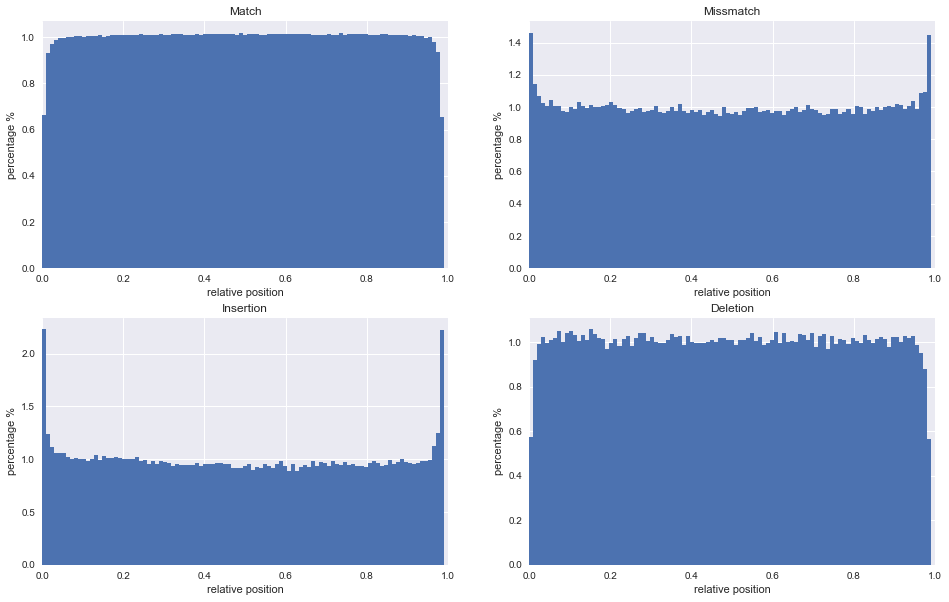
\includegraphics[width=0.7\textwidth]{./imgs/operation_distributed_r9.png}
		\caption{Cigar operations histogram over relative position inside read}
		\label{fg:cigar_op_dist}
	\end{center}
\end{figure}

\section{Consensus analysis}

%TODO ZAKLJUCAK
%%%%%%%%%%%%%%%%%%%%%%%%%%%%%%%%%%%%%%%%%%%%%%%%%%%%%%%%%%%%%%%%%%%%%%%%%%%%%%%%%%%%%%%
%% CHAPTER
\chapter{Conclusion}
Conclusion.



%TODO ABSTRACTS
%%%%%%%%%%%%%%%%%%%%%%%%%%%%%%%%%%%%%%%%%%%%%%%%%%%%%%%%%%%%%%%%%%%%%%%%%%%%%%%%%%%%%%%
%% DONE
\bibliography{references}
\bibliographystyle{unsrtnat}
\begin{abstract}
Abstract.

\keywords{Keywords.}
\end{abstract}

\hrtitle{Model dubokog učenja za određivanje očitanih baza dobivenih uređajem za sekvenciranje MinION}
\begin{sazetak}
Sažetak na hrvatskom jeziku.

\kljucnerijeci{Ključne riječi, odvojene zarezima.}
\end{sazetak}

\end{document}
